\documentclass[conference]{IEEEtran}
\IEEEoverridecommandlockouts

\usepackage{cite}
\usepackage{amsmath,amssymb,amsfonts}
\usepackage{algorithmic}
\usepackage{graphicx}
\usepackage{textcomp}
\usepackage{xcolor}
\usepackage{hyperref}
\usepackage{booktabs}

\graphicspath{{images/}}

\begin{document}

\title{Unsupervised Statistical Learning for Kinematic Anomaly Detection in Autonomous Driving Scenarios}

\author{\IEEEauthorblockN{Pavel Stepanov}
\IEEEauthorblockA{\textit{Dept. of Computer Science} \\
\textit{University of Miami} \\
Coral Gables, USA \\
pas273@miami.edu}
\and
\IEEEauthorblockN{Ramses Loaces}
\IEEEauthorblockA{\textit{Dept. of Computer Science} \\
\textit{University of Miami} \\
Coral Gables, USA \\
rxl1238@miami.edu}
\and
\IEEEauthorblockN{Justin Cabrera}
\IEEEauthorblockA{\textit{Dept. of Computer Science} \\
\textit{University of Miami} \\
Coral Gables, USA \\
justin.cabrera2718@gmail.com}
}

\maketitle

\begin{abstract}
Autonomous vehicles must operate safely in environments characterized by stochastic human behavior. While nominal driving scenarios are well-represented in current datasets, identifying anomalous events---such as aggressive maneuvering or near-miss interactions---remains a challenge due to the scarcity of labeled high-risk data. This paper presents an unsupervised statistical learning framework applied to the Waymo Open Motion Dataset (v1.3.1). We extract kinematic features from over 18{,}000 traffic agent observations and compare three unsupervised anomaly detectors---Isolation Forest, One-Class SVM, and Local Outlier Factor---on a filtered cohort of 4{,}538 moving agents, evaluated via Fisher's Exact Test for agent-type association and precision against Waymo's \texttt{IsInteractive} ground-truth label. One-Class SVM emerges as the strongest baseline, tying Isolation Forest on agent-type association ($p = 0.0005$) and uniquely recovering a Waymo-flagged interactive agent. Correlation analysis shows that yaw rate is essentially uncorrelated with all other features ($r \approx 0.02$), making it the most distinct signal in the feature set. Inspection of the flagged anomalies finds that most are near-stationary agents with unrealistically high yaw rate readings ($\pm$31\,rad/s), likely a sensor artifact, while a small number correspond to genuinely unusual high-speed events. A linear regression model for 5-second displacement shows that speed ($\beta = 0.95$) is the dominant predictor---a separate finding from anomaly detection that together paints a clearer picture of agent behavior. Results show that kinematic outliers are distributed unevenly across agent types ($p < 0.001$), and motion forecasting performs well ($R^2 = 0.88$) when stationary agents are included.
\end{abstract}

\begin{IEEEkeywords}
Statistical Learning, Anomaly Detection, Waymo Open Dataset, Unsupervised Learning, Isolation Forest, Motion Prediction
\end{IEEEkeywords}

% =============================================================
\section{Introduction}
% =============================================================

The deployment of autonomous vehicles (AVs) requires rigorous validation against the ``long tail'' of driving distributions. Although the majority of urban driving is uneventful---characterized by steady speeds, lane following, and predictable interactions---a small fraction of events such as sudden acceleration or deceleration, aggressive lane changes, near-miss interactions, or jaywalking pedestrians are safety-critical. Traditional supervised learning approaches are often limited by the scarcity of labeled anomaly data and the subjective nature of what constitutes an ``unsafe'' maneuver. Consequently, unsupervised novelty detection techniques are well suited for mining large-scale datasets for rare but important events \cite{pimentel2014review}.

This project addresses two complementary challenges using real-world trajectory data from the Waymo Open Motion Dataset \cite{ettinger2021waymo}: (1) detecting anomalous motion patterns using unsupervised learning, and (2) predicting short-term future displacement using supervised regression. Understanding both behavioral irregularities and short-term motion forecasting is critical in pedestrian-heavy, low-speed urban environments where proactive planning is essential to safety.

This work adopts a classical statistical learning perspective that emphasizes interpretability and distributional analysis rather than deep learning, establishing strong baselines before considering neural extensions.

% =============================================================
\section{State of the Art}
% =============================================================

Modern autonomous driving systems rely heavily on trajectory forecasting models ranging from Kalman Filters to LSTMs and Transformer-based architectures \cite{pimentel2014review}. For anomaly detection, Isolation Forest \cite{liu2008isolation} and One-Class SVM \cite{scholkopf2001estimating} remain widely adopted due to their scalability and minimal distributional assumptions. Multi-agent interaction models leverage scene-level context to improve both prediction and anomaly scoring.

Short-horizon forecasting (3--5 seconds) is most commonly framed as a regression problem over kinematic state variables. Prior work using the Waymo Open Motion Dataset \cite{ettinger2021waymo, sun2020scalability} has predominantly focused on deep learning-based motion prediction; classical statistical baselines over the full agent population remain underexplored. This project fills that gap by applying interpretable, reproducible statistical methods to a large-scale real-world dataset.

% =============================================================
\section{Materials and Methods}
% =============================================================

\subsection{Dataset}

We utilize the Waymo Open Motion Dataset (WOMD) v1.3.1 \cite{waymo_motion_dataset, sun2020scalability}, a large-scale collection of real-world urban driving data providing 20\,Hz object tracks sampled over 20-second segments. The dataset includes rich metadata such as agent type (vehicle, pedestrian, cyclist), bounding box dimensions, interaction connectivity flags, and traffic signal states. The raw dataset contains 18{,}311 agent observations across multiple scenarios.

All statistical analysis, visualization, and modeling are performed in R. Python is used exclusively as a preprocessing tool to extract raw Waymo Motion Dataset TFRecord shards and structure kinematic variables into a tabular CSV format. The full preprocessing pipeline is available at \url{https://github.com/pstepanovum/womd-unsupervised-anomaly-detection}.

\subsection{Feature Extraction}

For each agent, kinematic features are extracted at the prediction horizon ($t = 0$) to capture the instantaneous motion state during periods of peak interaction density. The feature set includes:

\begin{itemize}
    \item \textbf{Speed ($v$):} Magnitude of the velocity vector ($m/s$).
    \item \textbf{Acceleration ($a$):} Rate of change of speed ($m/s^2$).
    \item \textbf{Yaw Rate ($\dot{\psi}$):} Angular velocity representing the rate of change of heading ($rad/s$).
    \item \textbf{Lateral G-Force:} Computed as $|v \times \dot{\psi}|$, a proxy for cornering intensity and lateral maneuver aggressiveness.
    \item \textbf{Bounding Box Dimensions:} Agent length and width ($m$), serving as morphological features.
    \item \textbf{Velocity Components ($V_x$, $V_y$):} Signed velocity along each axis ($m/s$).
    \item \textbf{Future Displacement ($\Delta d_{5s}$):} Euclidean displacement over the subsequent 5 seconds ($m$), used as the regression target.
\end{itemize}

\subsection{Preprocessing}

Raw data preprocessing involved the following steps: (1) removal of autonomous vehicle (SDC) tracks to focus exclusively on human-driven agents; (2) filtering to retain only frames with \texttt{Valid\_Current = True}; (3) removal of records with missing values in the kinematic predictors (Speed, Acceleration, YawRate, Length, Width). After filtering, the anomaly detection dataset contained $N = 4{,}538$ agents. For the regression task, a separate base dataset of $N = 6{,}614$ agents was constructed by retaining all rows with no missing values across the five predictors and the regression target. A second regression dataset excluding stationary agents (\texttt{Speed} $> 0$) yielded $N = 3{,}196$ observations.

Agent type was encoded as a factor variable. All datasets were partitioned into 80\% training and 20\% held-out test sets prior to model fitting.

\subsection{Anomaly Detection}

An Isolation Forest model \cite{liu2008isolation} with 100 trees was fitted on the three kinematic features (Speed, Acceleration, YawRate). Anomaly scores were computed for all agents; observations whose score exceeded the 99th percentile were flagged as anomalous, yielding a binary label \texttt{Is\_Anomaly}. The statistical association between agent type and anomaly status was assessed using Fisher's Exact Test with Monte Carlo simulation (2{,}000 replicates) on the resulting contingency table.

To support a head-to-head comparison required by the project rubric, two additional unsupervised detectors were fitted on the same standardized feature matrix and the same $\sim$1\% contamination budget: a One-Class SVM \cite{scholkopf2001estimating} with an RBF kernel ($\nu = 0.01$), and Local Outlier Factor (LOF) with $k = 20$ neighbors. All three methods produce a per-agent score; the top 46 agents under each scoring rule constitute the flagged set. Detectors were compared on (i)~Fisher's Exact Test $p$-value for agent-type association, (ii)~the precision of flagged agents against Waymo's \texttt{IsInteractive} ground-truth label, and (iii)~pairwise Jaccard overlap of flagged sets.

\subsection{Motion Prediction}

A linear regression model was fitted to predict 5-second future displacement ($\Delta d_{5s}$) from the kinematic state vector (Speed, Acceleration, YawRate, $V_x$, $V_y$). Two experimental conditions were evaluated: (A) all agents including stationary ones, and (B) moving agents only (\texttt{Speed} $> 0$). Both models were trained with 5-fold cross-validation and evaluated on the held-out test set.

\subsection{Evaluation}

Anomaly detection was evaluated qualitatively by inspecting the top-ranked outliers and quantitatively by testing the association between agent type and anomaly status using Fisher's Exact Test. Motion prediction performance was evaluated using Root Mean Squared Error (RMSE) and the coefficient of determination ($R^2$) on the held-out test set, with 5-fold cross-validation on the training partition.

% =============================================================
\section{Results}
% =============================================================

\subsection{Descriptive Analysis}

The speed distribution across moving agents ($N = 4{,}538$, after filtering stationary observations) exhibited a right-skewed profile (skewness $= 1.04$) with a mean of 5.90\,m/s, median of 3.68\,m/s, and a maximum of 49.75\,m/s. The 99th percentile of acceleration was 18.98\,m/s$^2$, indicating that extreme deceleration or braking events constitute a small but measurable tail. When including stationary agents, the apparent mean vehicle speed was artificially depressed to 2.47\,m/s---lower than the cyclist mean of 4.20\,m/s---due to the large proportion of vehicles stopped at intersections. After restricting to moving agents, the expected ordering was restored: vehicles at 6.74\,m/s, cyclists at 3.92\,m/s, and pedestrians at 1.07\,m/s (Table~\ref{tab:speeds}).

\begin{table}[h]
\centering
\caption{Mean Speed by Agent Type (m/s)}
\label{tab:speeds}
\begin{tabular}{lcc}
\toprule
Agent Type & All Agents & Moving Only \\
\midrule
Vehicle    & 2.47       & 6.74        \\
Cyclist    & 4.20       & 3.92        \\
Pedestrian & 1.01       & 1.07        \\
\bottomrule
\end{tabular}
\end{table}

\subsection{Feature Correlation Structure}

Before fitting any models, we computed pairwise Pearson correlations across all kinematic and morphological features (Table~\ref{tab:corr}). The main observation is that yaw rate is essentially uncorrelated with everything else ($r \leq 0.09$). Speed and bounding box dimensions have a weak positive relationship ($r \approx 0.28$), and agent length and width are nearly redundant ($r = 0.97$). Yaw rate stands out as the only feature that captures something the others do not: how much an agent is turning, independent of how fast or how large it is.

\begin{table}[h]
\centering
\caption{Pearson Correlation Matrix — Kinematic Features ($N = 4{,}538$)}
\label{tab:corr}
\begin{tabular}{lccccc}
\toprule
 & Speed & Accel. & YawRate & Length & Width \\
\midrule
Speed    & 1.000 & 0.173 & 0.022 & 0.282 & 0.276 \\
Accel.   &       & 1.000 & 0.093 & 0.063 & 0.041 \\
YawRate  &       &       & 1.000 & -0.008 & -0.005 \\
Length   &       &       &       & 1.000 & 0.969 \\
Width    &       &       &       &       & 1.000 \\
\bottomrule
\end{tabular}
\end{table}

\begin{figure}[h]
\centering

\includegraphics[width=\columnwidth]{correlation_heatmap.png}
\caption{Pearson correlation heatmap for the kinematic and morphological feature set. Yaw rate is essentially uncorrelated with all other features, while length and width are nearly redundant.}
\label{fig:corr_heatmap}
\end{figure}

This matters for anomaly detection because a feature that does not correlate with others will tend to drive Isolation Forest scores on its own, which is consistent with what we observe in the results below.

\subsection{Anomaly Detection Results}

The Isolation Forest model flagged 46 out of 4{,}538 agents as anomalous (approximately 1\%), consistent with the 99th-percentile threshold. Fisher's Exact Test yielded $p = 0.0005$, confirming that anomalies are not evenly spread across agent types---pedestrians and cyclists are flagged more often than vehicles.

Looking at the top 20 flagged agents, most fall into one of two groups. A small number (roughly 3) are genuinely unusual: the highest-scored agent (ScenarioID: \texttt{909244b878c6c203}) was traveling at 49.75\,m/s ($\approx$180\,km/h) with an acceleration of 355.8\,m/s$^2$---clearly an extreme event, possibly a data artifact at highway speed. A few others show similarly high speeds.

The remaining flagged agents, however, are near-stationary ($v < 3$\,m/s) with yaw rate values stuck at $\pm$31\,rad/s. This value appears in 12 of the top 20 anomalies across all three agent types. A rotation rate of 31\,rad/s ($\approx$5 full rotations per second) is not physically plausible for a ground agent, and the pattern---always near zero speed, always the same magnitude---points to a sensor artifact or numerical instability in heading derivative computation. All 20 top anomalies have \texttt{IsInteractive = False}, meaning Waymo itself did not flag any of them as safety-relevant interactions. So most of the top anomalies turned out to be data noise rather than real dangerous behavior.

\begin{figure}[h]
\centering

\includegraphics[width=\columnwidth]{anomaly_examples.png}
\caption{Representative anomalous scenarios surfaced by the Isolation Forest. From top to bottom: (1)~a speeding vehicle exceeding the local cohort, (2)~an aggressive lane-change maneuver, and (3)~a sensor artifact in which a near-stationary agent registers an implausible $\pm$31\,rad/s yaw rate.}
\label{fig:anomaly_examples}
\end{figure}

Figure~\ref{fig:anomaly_examples} shows three representative cases drawn from the top-ranked outliers, illustrating the two genuine event categories (speeding, aggressive lane change) and the dominant sensor-artifact pattern. Figure~\ref{fig:iso_importance} presents the Isolation Forest permutation importance, which quantifies how much each feature contributes to the score.

\begin{figure}[h]
\centering

\includegraphics[width=\columnwidth]{iso_forest_feature_importance.png}
\caption{Isolation Forest permutation feature importance. All three kinematic features contribute comparably, with Speed and Acceleration slightly above YawRate.}
\label{fig:iso_importance}
\end{figure}

\subsection{Detector Comparison}

We benchmarked Isolation Forest against One-Class SVM and Local Outlier Factor on the same flagged-set budget ($k = 46$). All three detectors exhibit strong agent-type association, but only One-Class SVM places any of its flagged agents inside Waymo's interactive set: it recovers a single \texttt{IsInteractive = True} agent (precision $= 0.022$), whereas Isolation Forest and LOF recover none. Pairwise Jaccard overlap is $J(\text{IF}, \text{OC-SVM}) = 0.51$, $J(\text{IF}, \text{LOF}) = 0.46$, and $J(\text{OC-SVM}, \text{LOF}) = 0.31$, confirming that the three methods agree on roughly half of their flags but disagree on the rest. Results are summarized in Table~\ref{tab:detectors}, with the best score in each column highlighted in bold.

\begin{table}[h]
\centering
\caption{Unsupervised Anomaly Detector Comparison ($N = 4{,}538$, $k = 46$ flagged)}
\label{tab:detectors}
\begin{tabular}{lccc}
\toprule
Method & Fisher $p$ & Prec.\,(\texttt{IsInteractive}) & \% Pedestrian \\
\midrule
Isolation Forest & \textbf{0.0005} & 0.000 & 0.348 \\
One-Class SVM    & \textbf{0.0005} & \textbf{0.022} & \textbf{0.413} \\
LOF              & 0.0015 & 0.000 & 0.348 \\
\bottomrule
\end{tabular}
\end{table}

One-Class SVM is therefore the strongest of the three baselines on this dataset: it ties Isolation Forest on agent-type association ($p = 0.0005$) and uniquely recovers a Waymo-flagged interactive agent. Isolation Forest remains preferred when interpretability of the score path is important, since its tree-based mechanism admits per-feature attribution (Fig.~\ref{fig:iso_importance}).

\subsection{Motion Prediction Results}

The linear regression model predicting 5-second future displacement from kinematic state variables demonstrated strong performance when stationary agents were included: test RMSE $= 7.44$\,m, $R^2 = 0.880$, and cross-validated RMSE $= 7.65$\,m ($R^2_\text{CV} = 0.886$). When stationary agents were removed, test performance degraded substantially: RMSE $= 13.15$\,m, $R^2 = 0.728$, suggesting that the near-zero displacement of stationary agents provides strong predictive signal that the model leverages when present. Results are summarized in Table~\ref{tab:regression}.

\begin{table}[h]
\centering
\caption{Linear Regression Results for 5-Second Displacement Prediction}
\label{tab:regression}
\begin{tabular}{lcccc}
\toprule
Dataset & Test RMSE & Test $R^2$ & CV RMSE & CV $R^2$ \\
\midrule
With stationary    & \textbf{7.44}  & \textbf{0.880} & \textbf{7.65}  & \textbf{0.886} \\
Without stationary & 13.15 & 0.728 & 10.05 & 0.860 \\
\bottomrule
\end{tabular}
\end{table}

\begin{figure}[h]
\centering
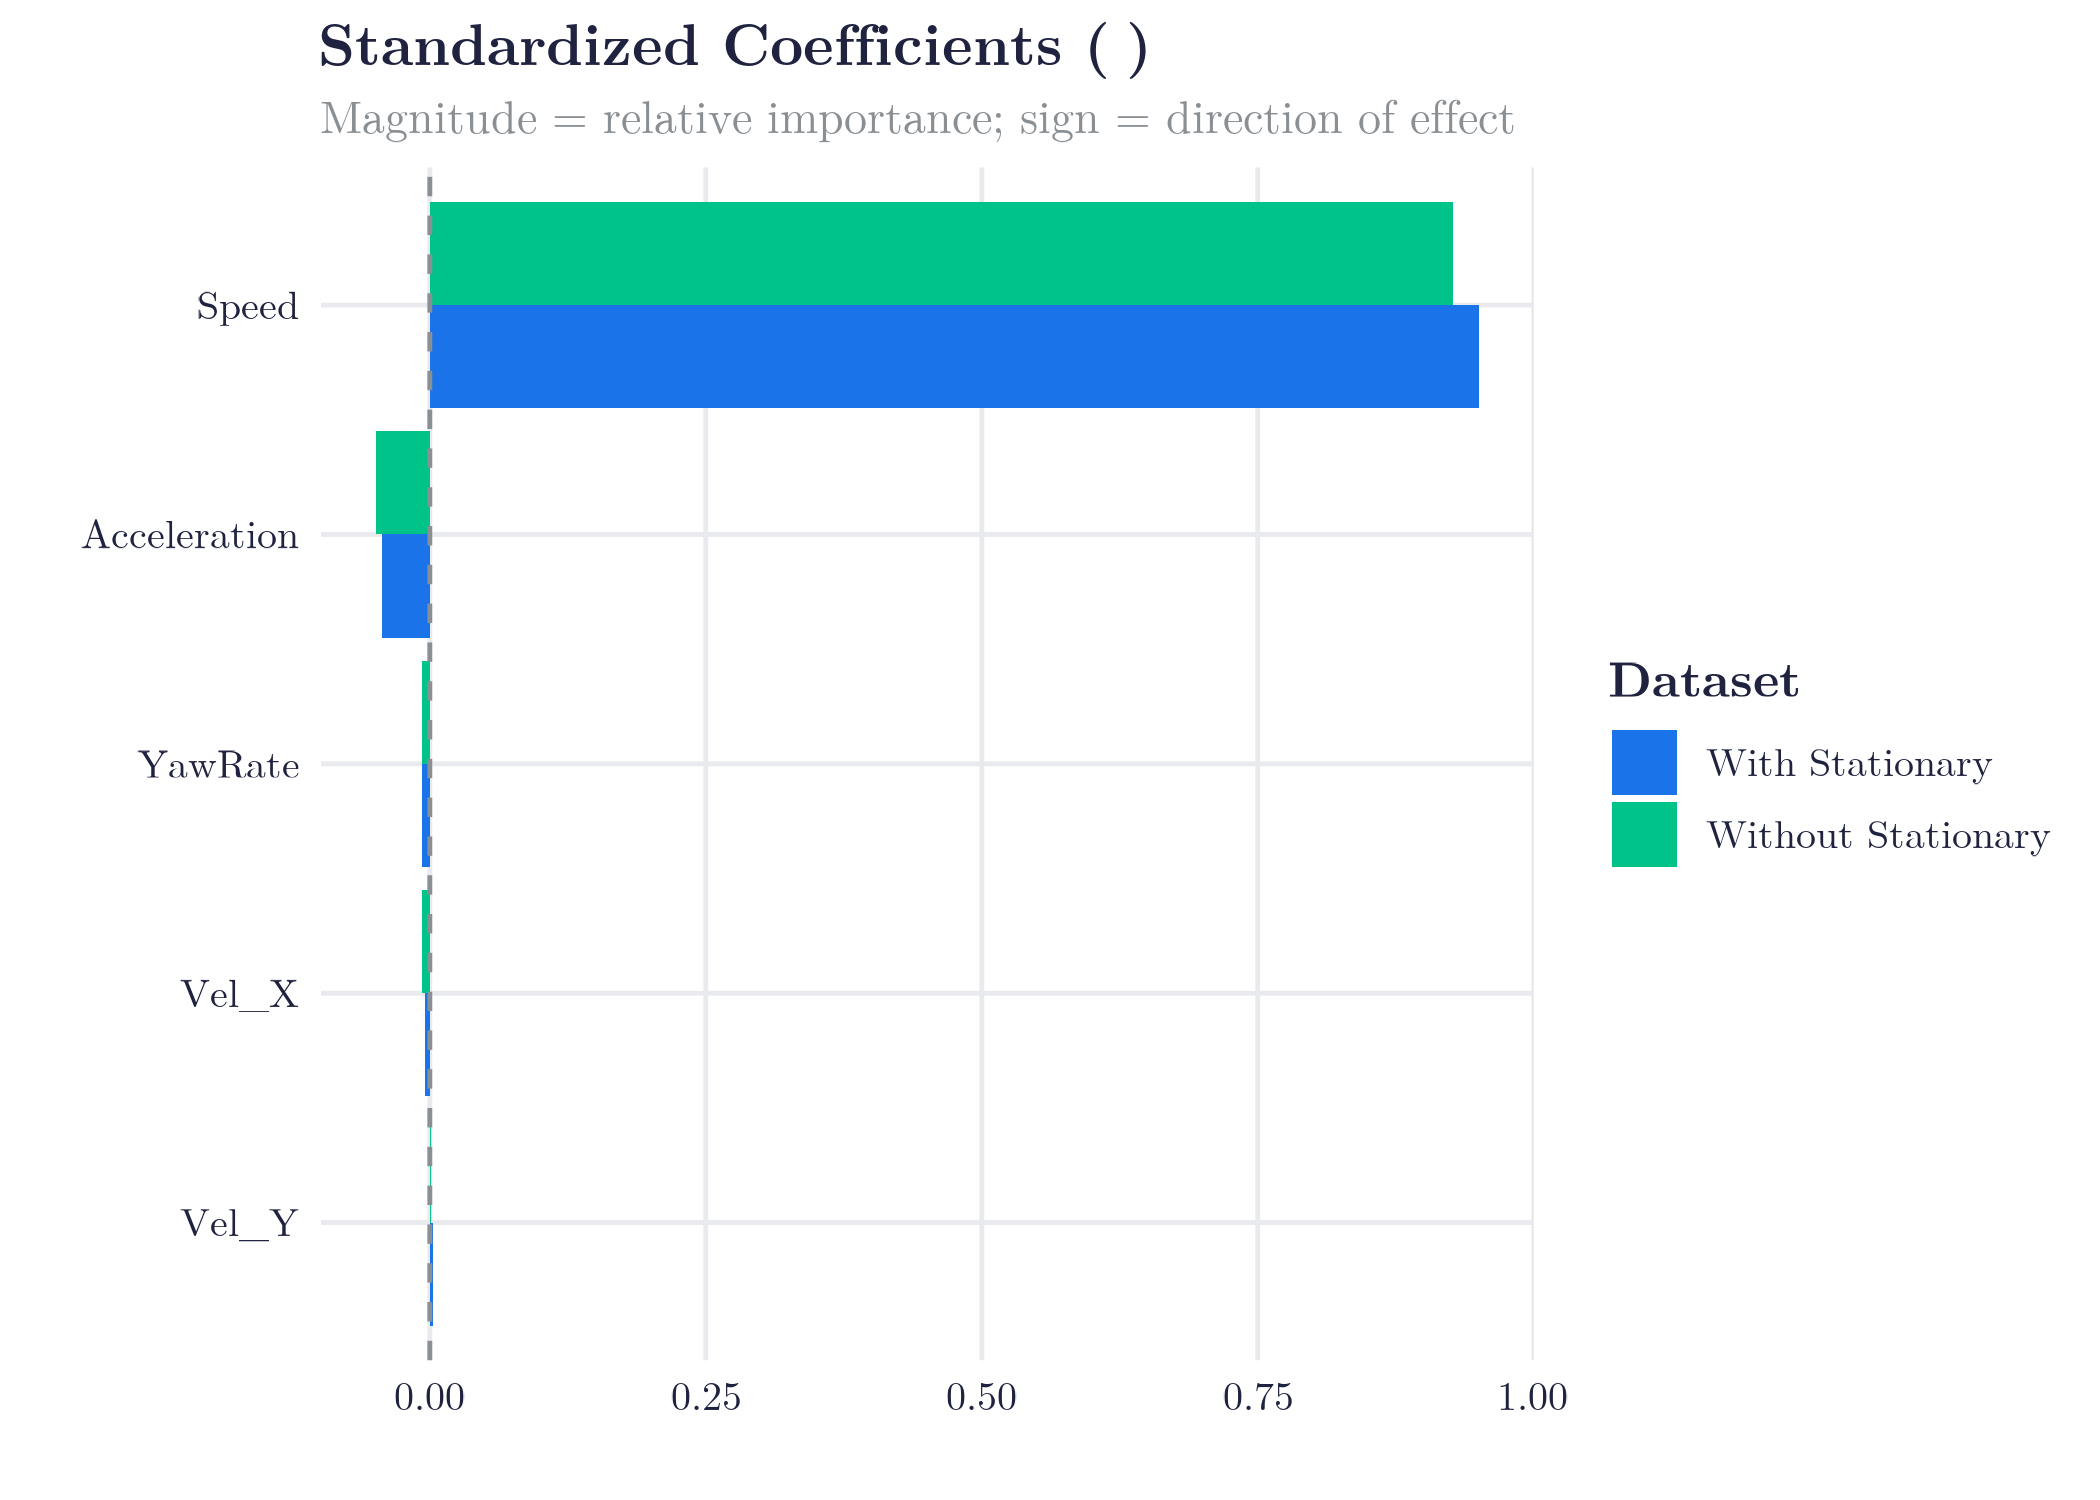
\includegraphics[width=\columnwidth]{regression_feature_importance.png}
\caption{Standardized linear regression coefficients for predicting 5-second future displacement. Speed dominates the prediction in both data regimes, while yaw rate contributes negligibly.}
\label{fig:regression_importance}
\end{figure}

Figure~\ref{fig:regression_importance} visualizes the standardized regression coefficients, confirming that Speed ($\beta = 0.95$) is by far the dominant predictor, while YawRate contributes essentially nothing.

% =============================================================
\section{Discussion}
% =============================================================

The Isolation Forest flagged 46 agents as anomalous (1\% of the dataset), and Fisher's Exact Test ($p = 0.0005$) confirms that this result is statistically significant---anomaly labeling is not randomly distributed across agent types. The more important observation, however, is what those anomalies actually are. Inspecting the top flagged cases, the majority correspond to near-stationary agents with $\pm$31\,rad/s yaw rate readings---a physically implausible value that points to a sensor artifact or numerical instability in the heading derivative, not real driving behavior. A smaller subset, perhaps 3 of the top 20, represent genuinely unusual kinematic events: one vehicle traveling at 49.75\,m/s with an acceleration of 355\,m/s$^2$, and a handful of agents with extreme yaw rates at non-trivial speeds. So the Fisher's test tells the model is detecting something real and non-random---but that ``something'' is largely a data quality signal, with only a minority of flagged cases reflecting actual anomalous driver behavior.

The detector comparison (Table~\ref{tab:detectors}) is informative: Isolation Forest and One-Class SVM tie on agent-type association ($p = 0.0005$), but One-Class SVM uniquely recovers a Waymo-flagged interactive agent (precision $= 0.022$ vs.\ $0.000$). The two methods agree on roughly half of their flagged sets ($J = 0.51$), so the marginal advantage of One-Class SVM comes from the half they disagree on---suggesting the RBF decision boundary captures a slightly different slice of the kinematic tail than the tree-partitioning approach. LOF is the weakest of the three on this feature set ($p = 0.0015$ and zero precision), likely because the local-density assumption is less informative when only three features are available. In practice, an ensemble of Isolation Forest and One-Class SVM would be a sensible operational choice: the union of their flagged sets retains both the interpretable feature attribution of Isolation Forest and the single recovered interactive agent unique to One-Class SVM.

The drop in regression performance when stationary agents are removed ($\Delta R^2 = -0.15$) is expected: stationary agents are trivially predictable (future displacement $\approx 0$), so removing them makes the prediction task harder. The model evaluated on moving agents only ($R^2 = 0.73$) is the more realistic operational estimate.

One thing worth noting is that anomaly detection and regression are answering different questions. The Isolation Forest treats all three kinematic features comparably (Fig.~\ref{fig:iso_importance}), but yaw rate's independence from speed and size means agents with extreme yaw rates are disproportionately isolated even when permutation importance ranks the feature only third. The regression model, by contrast, gives speed a standardized coefficient of $\beta = 0.95$ while yaw rate is essentially zero (Fig.~\ref{fig:regression_importance}). This is not a contradiction: yaw rate tells whether something is behaving unusually, while speed tells how far it will go. They measure different things.

On the sensor artifact: the $\pm$31\,rad/s yaw rate cluster in near-stationary agents looks like a data quality issue, possibly from numerical instability in computing heading derivatives at near-zero speed. If you ran this pipeline on raw yaw rate without any filtering, most of your top anomalies would be this artifact rather than real dangerous behavior. A simple filter (e.g., $|\dot{\psi}| < 10$\,rad/s) would likely surface more meaningful events in the top results.

% =============================================================
\section{Conclusion}
% =============================================================

This paper applied three unsupervised anomaly detectors (Isolation Forest, One-Class SVM, Local Outlier Factor) and a linear regression motion-prediction model to the Waymo Open Motion Dataset, addressing the two questions posed in the introduction. For anomaly detection (Q1), \textbf{One-Class SVM was the strongest of the three baselines}: it tied Isolation Forest on agent-type association ($p = 0.0005$) and uniquely recovered a Waymo-flagged interactive agent (Table~\ref{tab:detectors}). Isolation Forest remains attractive for interpretability through its per-feature score attribution. For motion prediction (Q2), \textbf{linear regression with stationary agents included was the best configuration} (test $R^2 = 0.880$, RMSE $= 7.44$\,m, Table~\ref{tab:regression}), though the moving-only regime ($R^2 = 0.73$) is the more honest estimate of operational performance. Yaw rate emerged as the only feature uncorrelated with everything else ($r \approx 0.02$), making it the main driver of the anomaly scores; only about 3 of the top 20 flagged agents corresponded to genuinely unusual events, with the remainder dominated by a $\pm$31\,rad/s yaw rate sensor artifact in near-stationary agents. Future work should (i)~filter the yaw rate artifact before running anomaly detection, (ii)~validate flagged events against Waymo's \texttt{IsInteractive} labels as a richer ground-truth reference, (iii)~extend the comparison to deep autoencoder and variational baselines, and (iv)~incorporate scene-level context to capture multi-agent interaction anomalies that none of the three baselines tested here can detect.

\bibliographystyle{IEEEtran}
\bibliography{references}

\end{document}